%! TeX program = lualatex
\documentclass[]{beamer} 

\setbeamercolor{title}{fg=black}
\setbeamercolor{frametitle}{fg=black}
\setbeamercolor{caption}{fg=black}
\setbeamercolor{caption name}{fg=black}

\setbeamertemplate{navigation symbols}{}
\setbeamertemplate{itemize item}{\color{black}$\bullet$}

% packages
\usepackage{fontspec}
\setmainfont{EB Garamond}
\usefonttheme{serif}
\setmonofont[Scale=MatchLowercase]{Deja Vu Sans Mono}

\usepackage{microtype}      % Slightly tweak font spacing for aesthetics
\usepackage[english]{babel} % Language hyphenation and typographical rules

\usepackage{minted}
\usemintedstyle{algol_nu}
\usepackage{xcolor}

\usepackage{pgfplots}
\pgfplotsset{width=\textwidth,compat=1.9}

\usepackage{caption}
\newenvironment{code}{\captionsetup{type=listing, skip=0pt}}{}

\usepackage[yyyymmdd]{datetime}
\renewcommand{\dateseparator}{--}

\usepackage{titlesec}

\author{Andrew Hayes (ID: 21321503)}
\title{Why Vim is My Favourite Text Editor}
\subtitle{CT3112 Professional Skills: Assignment 01}
\institute{University of Galway}

\begin{document}

\titlegraphic{
\includegraphics[width=3cm]{./images/vim_logo.png}}
\frame{\titlepage}

\begin{frame}{Introduction}
    By the end of this presentation, I intend for you to have gained an understanding of:
    \begin{itemize}
        \item   What Vim is and how it works.
        \item   The benefits of Vim.
        \item   The drawbacks of Vim.
        \item   Why I prefer Vim for all my text-editing work.
        \item   Whether or not Vim might be the right text editor for you.
        \item   What alternatives there are to Vim.
        \item   How you can get started with Vim.
    \end{itemize}
\end{frame}

\begin{frame}{What is Vim?}
    \begin{itemize}
        \item   \textbf{Vim} is terminal-based, modal text editor released in 1991, designed to be minimal \& fast to
                use.
        \item   It has a number of fast, mnemonic keybindings that make typical text-editing tasks much faster.
        \item   A \textbf{terminal-based} text editor is a text-only editor that is ran from the command line or
                terminal.
        \item   A \textbf{modal} text editor is one in which there are a number of different \textbf{modes} that the 
                editor can be in at any one time. 
    \end{itemize}
\end{frame}

\begin{frame}
    \begin{figure}[h]
        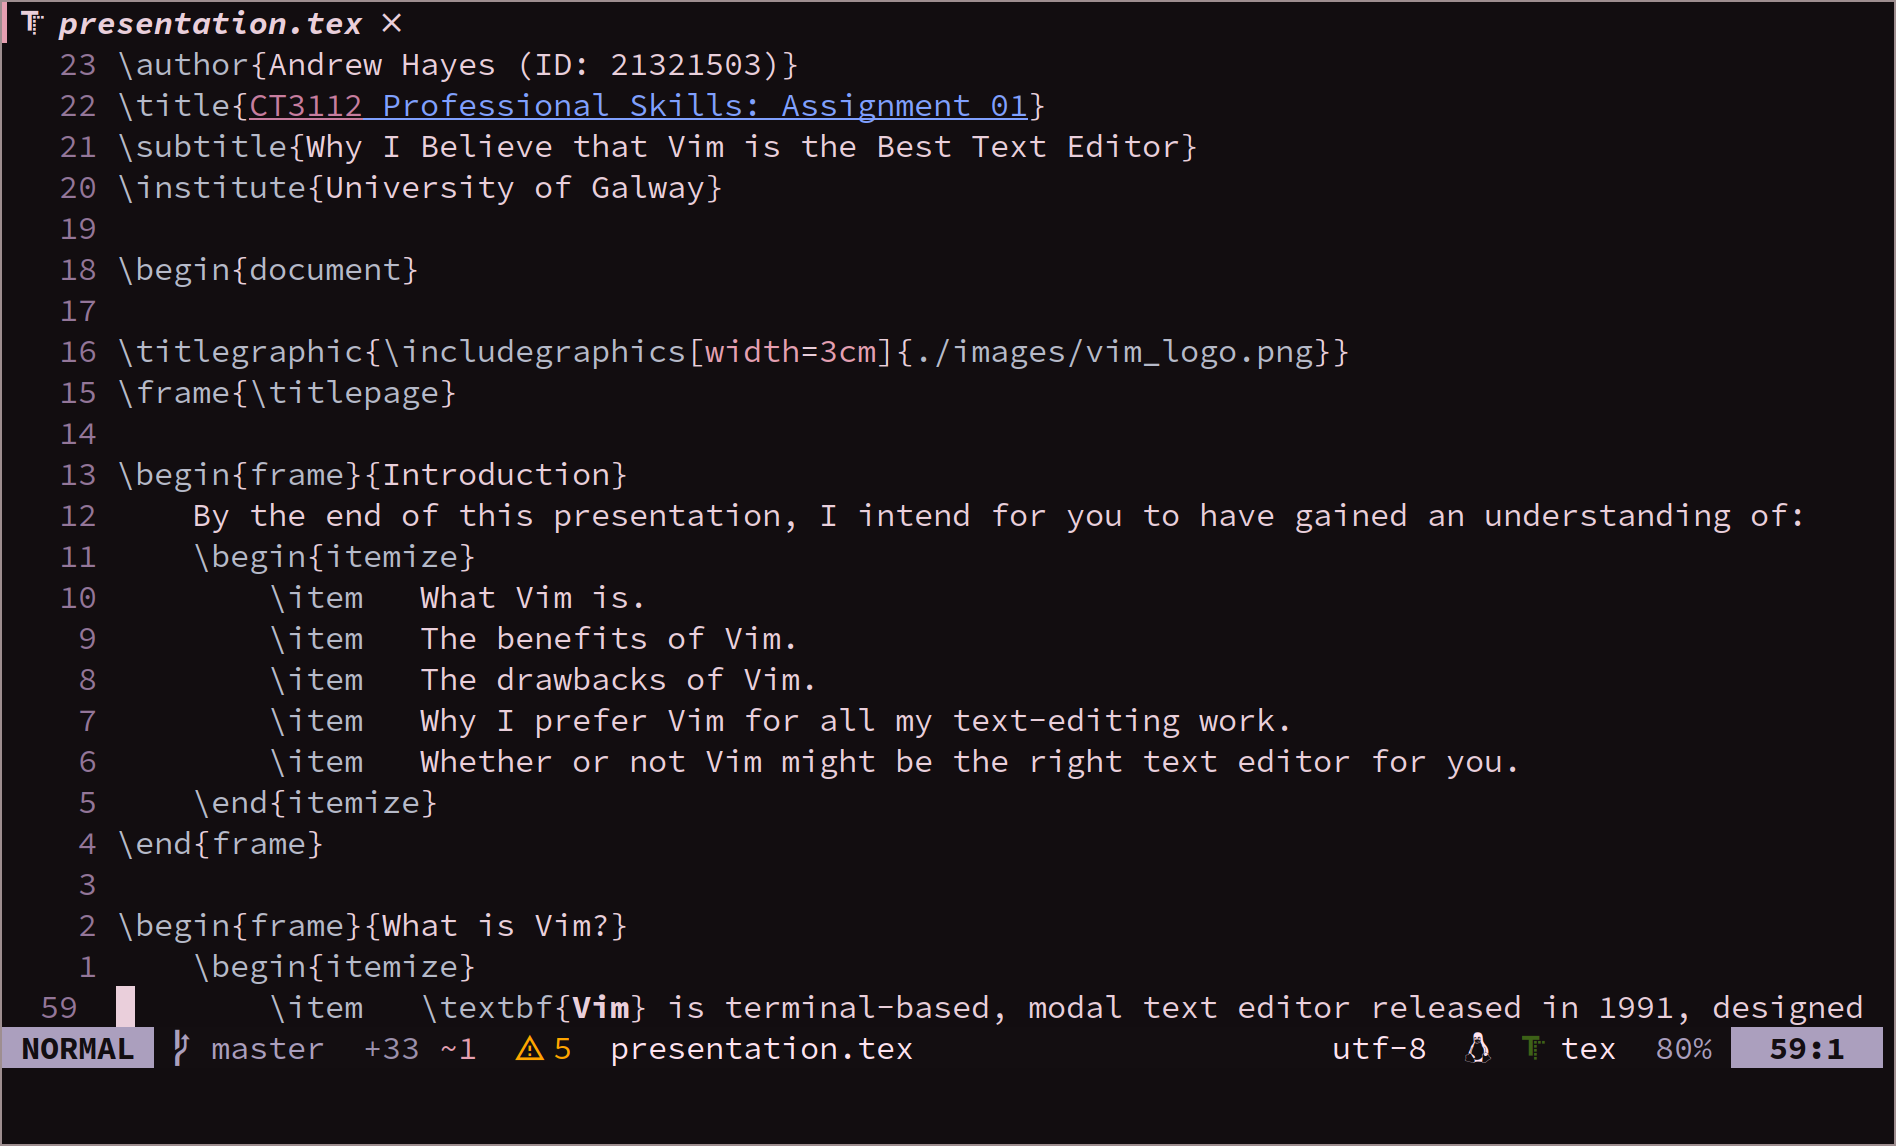
\includegraphics[width=\textwidth]{./images/screenshot.png}
        \caption{A Screenshot of Vim Being Used to Write this Presentation (in {\LaTeX})}
    \end{figure}
\end{frame}

\begin{frame}{What is a Terminal?}
    \begin{itemize}
        \item   A \textbf{terminal} is a text-based interface for a computer, originating from when computers did not
                have any graphics.
        \item   It is typically interacted with via a \textbf{command line}, where text commands are written to start
                programs.
        \item   To start Vim from the command line, simply type \mintinline{bash}{vim file_name.txt}
    \end{itemize}

    \begin{figure}[h]
        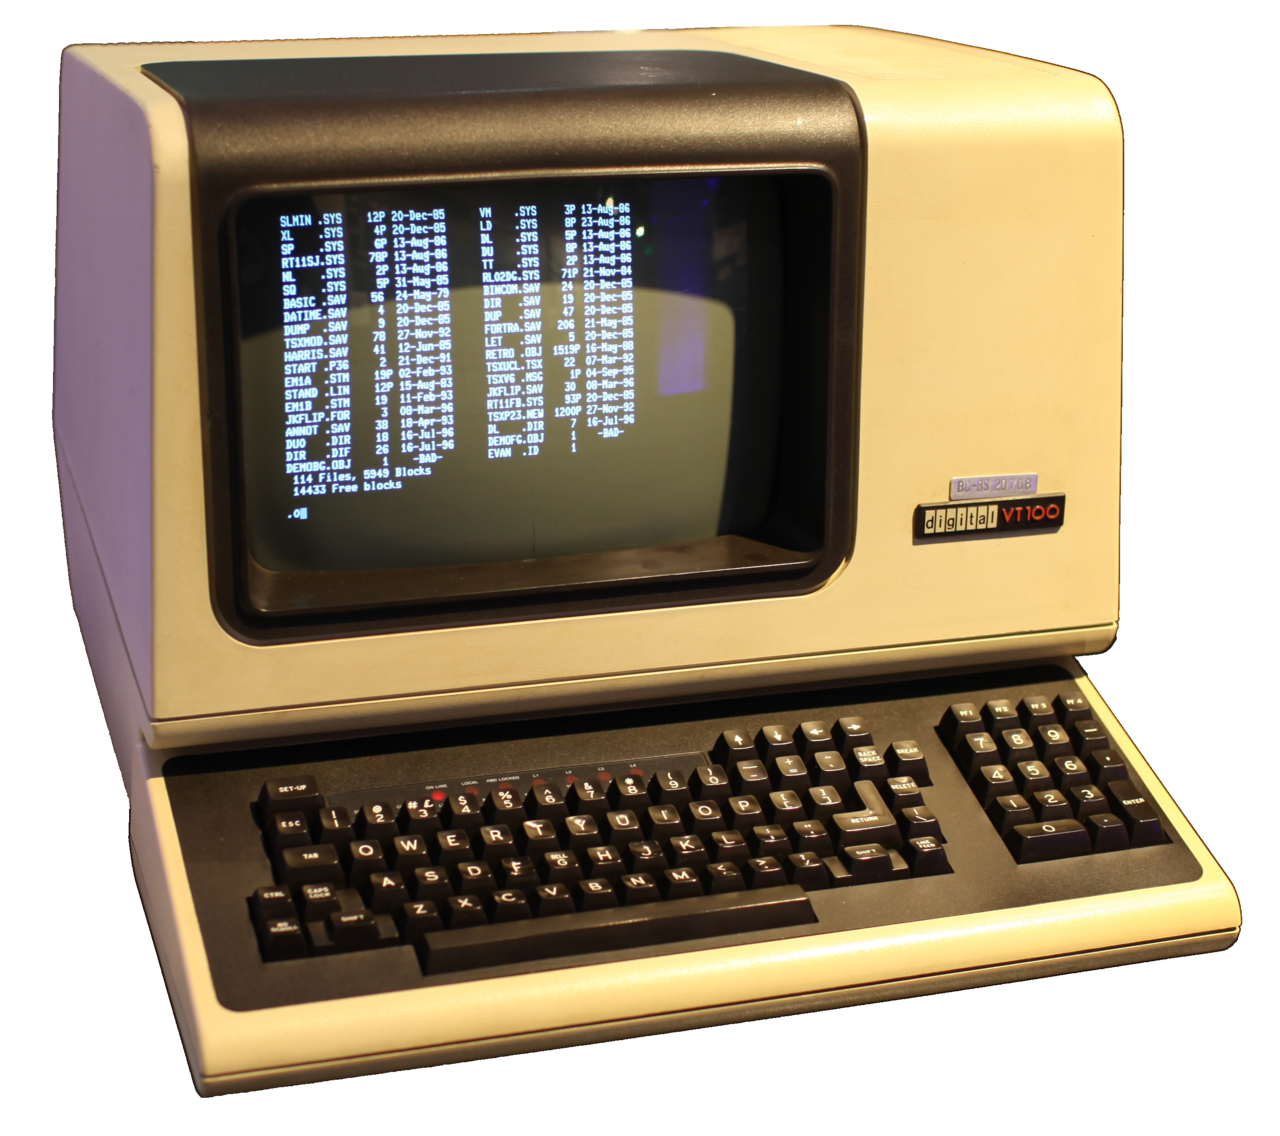
\includegraphics[width=0.4\textwidth]{./images/terminal.png}
        \caption{A Computer Terminal from 1978}
    \end{figure}
\end{frame}

\begin{frame}{What are the Vim Modes?}
    \begin{itemize}
        \item   \textbf{Normal mode} (\texttt{ESC}) is for the navigation \& manipulation of the text in the file
                being edited, via the shortcut keybindings.
                It is the default mode of the program.
        \item   \textbf{Insert mode} (\texttt{i}) is for inserting new text. This mode is similar to the
                default to the default behaviour of a more conventional text editor such as Notepad: text can be typed
                or removed with the backspace key, and navigation or selection can be done with the mouse or arrow
                keys.
        \item   \textbf{Visual mode} (\texttt{v}) is for the selection of text blocks for manipulation, with the
                selected text being highlighted, similar to selecting text with the mouse in other text editors.
                Visual mode has two sub-modes: \textbf{visual block} (\texttt{CTRL+v}) \& \textbf{visual line}
                (\texttt{V}), in which text can be selected either vertically by columns or horizontally by line.
    \end{itemize}
\end{frame}

\begin{frame}{What are the Vim keybindings?}
    \begin{itemize}
        \item   Too many to list here!
        \item   Navigation in normal mode can be done with the \texttt{hjkl} (direction) keys, which correspond to
                the left, down, up, \& right arrow keys respectively, allowing quick navigation without removing your
                fingers from the home row.
        \item   These direction keys can be combined with numbers to repeat them a certain number of times, e.g.:
                \texttt{5j} moves the cursor down 5 lines.
        \item   There are also a number of other direction keys: \texttt{w} to go forward a word of text, \texttt{b} to
                go back a word of text, \texttt{gg} to go to the start of the file, \texttt{G} to go to the end of the
                file.
    \end{itemize}
\end{frame}

\begin{frame}{What are the Vim keybindings?}
    \begin{itemize}
        \item   Vim keybindings typically take the form \textbf{action + direction}, i.e. the first key pressed
                indicates the action to be performed and the second key pressed indicates the direction in which to do
                it.
        \item   The most common action keys are \texttt{d} to delete text, \texttt{c} to change text, \texttt{y} to copy
                (or \textbf{yank}) text, and \texttt{p} to paste text.
        \item   The action keys are combined with direction keys, e.g. \texttt{dG} deletes all the text from the cursor
                to the end of the file, \texttt{y5w} copies the next 5 words to the clipboard, etc.
        \item   If you're trying to get the hang of Vim keybindings, the most important one for you to know is
                \texttt{u} to undo the last action you performed, in case you made a mistake!
    \end{itemize}
\end{frame}

\begin{frame}{What are the benefits of Vim?}
    \begin{itemize}
        \item   Lightweight \& minimal.
        \item   Speedy text editing with countless keybindings \& shortcuts.
        \item   Easy integration with other command-line programs.
        \item   Endlessly extensible through its configuration file (found at \mintinline{shell}{~/.vimrc})
        \item   Lots of community-developed plugins to extend its functionality even further.
        \item   It's very easy to quickly record a \textbf{macro} to perform an option repeatedly.
        \item   Standard on most modern UNIX-like systems; if you use a Linux-based system or MacOS, you likely already
                have it installed!
        \item   Most IDEs have a Vim mode, allowing you to use the Vim keybindings in many other programs too.
    \end{itemize}
\end{frame}

\begin{frame}{What are the drawbacks of Vim?}
    \begin{itemize}
        \item   Steep learning curve: there are so many keybindings that almost nobody knows them all.
        \item   No graphics support: because it's terminal-based, there is no way to display an image inside Vim.
        \item   Only works for plaintext editing: can't be used to edit Word documents or PowerPoint presentations.
        \item   Very minimal by default: it requires a lot of configuration to bring it to feature parity with a modern 
                IDE.
        \item   Requires some knowledge of the terminal: not suited for people who have no technical background.
    \end{itemize}
\end{frame}

\begin{frame}{Why I prefer Vim}
    \begin{itemize}
        \item   I spend most of my time on my computer editing plaintext code files, so the speed gained from using the 
                Vim keybindings is invaluable.
        \item   As a Linux user and programmer, I spend a lot of time in the terminal, so having a terminal-based editor 
                is very convenient for me.
        \item   Often for internship work, I will have to remotely connect to a server to edit its configurations and
                the only text editor available is Vim.
        \item   I enjoy the fine-grained control over the program's behaviour that the Vim configuration file affords
                me.
        \item   I think it looks cooler than other text editors!
    \end{itemize}
\end{frame}

\begin{frame}{Is Vim right for you?}
    \begin{itemize}
        \item   Vim is right for you if spend a lot of time editing plaintext files, using the terminal, or remotely
                accessing servers and you don't mind its steep learning curve. 
                If you want fine-grained control over the behaviour of your text editor, and the ability to endlessly
                extend it, then Vim is a good choice.
                It helps a lot if you have a technical background, but anyone can learn Vim!
        \item   Vim is not right for you if you rely heavily on graphical editors, e.g. Microsoft Word or PowerPoint, if
                you don't want to spend time learning the keybindings, or if you want a text editor that is feature-rich 
                out of the box without any customisation.
                If you rarely use the terminal in your day-to-day life, then a terminal-based text editor likely is not
                suitable for your workflow.
    \end{itemize}
\end{frame}

\begin{frame}{What alternatives are there to Vim?}
    Similar text editors to Vim include:
    \begin{itemize}
        \item   Emacs
        \item   Vi
        \item   Helix
        \item   Kakoune
    \end{itemize}

    More conventional text editors include:
    \begin{itemize}
        \item   Notepad
        \item   Atom
        \item   VSCode
        \item   Fully-featured IDEs such as Eclipse or Intellij.
    \end{itemize}
\end{frame}

\begin{frame}{How can I get started with Vim?}
    \begin{itemize}
        \item   Download \& install Vim from \url{https://www.vim.org/download.php}
        \item   Open a terminal emulator / command prompt on your computer.
        \item   Enter \texttt{vim file\_name.txt}, substituting \texttt{file\_name.txt} for the path to the file you
                want to edit / create, and start editing!
        \item   To get a more in-depth tutorial of how to use Vim, run the command \texttt{vimtutor} from your command
                prompt to start the tutorial.
    \end{itemize}
\end{frame}

\begin{frame}{Summary}
    By now, I hope that you have gained an understanding of:
    \begin{itemize}
        \item   What Vim is and how it works.
        \item   The benefits of Vim.
        \item   The drawbacks of Vim.
        \item   Why I prefer Vim for all my text-editing work.
        \item   Whether or not Vim might be the right text editor for you.
        \item   What alternatives there are to Vim.
        \item   How you can get started with Vim.
    \end{itemize}
\end{frame}

\end{document}
